\documentclass[iop]{emulateapj}

%Specify packages
\usepackage{amsmath}
\usepackage{subfigure}
%use for editing/highlighting
\usepackage{color,soul}

%Define new commands as needed
\newcommand{\ang}{\AA~}

\begin{document}
	%Frontmatter
	\title{``Hot'' Non-flaring Plasma in Active Regions II. Impacts of Two-fluid Effects}
	\author{W. T. Barnes}
	\author{S. J. Bradshaw}
	\affil{Department of Physics \& Astronomy, Rice University, Houston, TX 77251-1892}
	\email{will.t.barnes@rice.edu}
	\author{P. J. Cargill}
	\affil{Space and Atmospheric Physics, The Blackett Laboratory, Imperial College, London SW7 2BW}
	\affil{School of Mathematics and Statistics, University of St. Andrews, St. Andrews, Scotland KY16 9SS}
	
	%Abstract
	\begin{abstract}
		Faint, high-temperature emission in active region cores has long been predicted as a signature of nanoflare heating. However, the detection of such emission has proved difficult due to a combination of the efficiency of thermal conduction, non-equilibrium ionization, and inadequate instrument sensitivity. This second paper in our series on hot non-flaring plasma in active regions aims to show how the assumption of electron-ion equilibrium in hydrodynamic models leads to incorrect conclusions regarding the hot emission. We have used an efficient two-fluid hydrodynamic model to carry out a parameter exploration in preferentially heated species, nanoflare heating frequency, and event amplitude power-law index. By computing the emission measure distributions and calculating their ``hotward'' slopes, we have concluded that the assumption of electron-ion equilibrium leads to an understimate of the amount of hot plasma at intermediate and high heating frequencies. Additionally, in the single-fluid approximation, hot emission measure slopes show only a very weak dependence on heating frequency while in the electron-only heating scenario, the hotward slope varies more as the heating frequency increases. 
	\end{abstract}
	
	%Body
	\section{Introduction}
	\par\hl{Need to reword this introduction; move from introduction of hot plasma as signature of nanoflares to observational evidence for nanoflares and why it is hard to come by; to models which show evidence of nanoflares; to what we will do in this paper}
	%
	\par \citet{cargill_implications_1994,cargill_nanoflare_2004} have predicted that emission measure distributions resulting from nanoflare models should be wide and have a faint, high-temperature ($>4\times10^6$ K) component and thus a steep hotward slope. Unfortunately, observing this high-temperature emission is difficult and in some cases impossible. The reason for this difficulty is twofold. First, thermal conduction is a very efficient cooling mechanism at high temperatures and large spatial temperature gradients. Thus, because the increase in density lags the increase in temperature due to heating and because $\mathrm{EM}\propto n^2$, by the time sufficient densities are acheived, the plasma has cooled down such that the fingerprints of nanoflare heating have been smoothed out. 
	%
	\par The second reason for this difficulty is non-equilibrium ionization. It is usually assumed that the observed line intensities, because of their known formation temperatures, are a direct indicator of the plasma temperature. However, if the heating timescale is shorter than the ionization timescale, the time it takes for the ion population to settle into the correct charge state, an equilibrium assumption can lead to a misdiagnosis of the plasma temperature. This makes signatures of hot, nanoflare-heated plasma especially difficult to detect if the high temperatures persist for less than the ionization timescale \citep{bradshaw_explosive_2006,bradshaw_what_2011,reale_nonequilibrium_2008}.
	%
	\par Despite these difficulties, various attempts have been made to observe this faint high-temperature emission. Using the broadband X-Ray Telescope (XRT) aboard the \textit{Hinode} spacecraft, \citet{schmelz_hinode_2009} and \citet{reale_evidence_2009} show a faint hot component in the reconstructed $\mathrm{DEM}$ curves. However, since the channels on such broadband instruments can often be polluted by low-temperature emission, the reliability of such measurements depends on the filtering technique used. Additionally, \citet{winebarger_defining_2012} showed that combinations of \textit{Hinode}/EIS and \textit{Hinode}/XRT measurements leave a ``blind spot'' in the $\mathrm{EM}-T$ space conincident with where evidence for nanoflare heating is likely to be found. Unambiguous observational evidence of nanoflare heating must come from pure spectroscopic measurements \citep[see][]{brosius_pervasive_2014}. Missions like the Marshall Grazing Incidence X-ray Spectrometer (MaGIXS) \citep{kobayashi_marshall_2011,winebarger_new_2014}, with a wavelength range of 6-24 \ang and a temperature range of $6.2<\log{T}<7.2$, aim to probe this previously poorly-resolved portion of the coronal spectrum in hopes of better quantifying the presence of faint, high-temperature plasma.
	%
	\par The Parker nanoflare concept has become one of the most favored and contentious coronal heating models \citep{cargill_implications_1994,cargill_nanoflare_2004,klimchuk_solving_2006}. While many theoretical efforts \citep[e.g.][]{bradshaw_diagnosing_2012,reep_diagnosing_2013} have shown the feasability of nanoflares, the idea has long suffered from a lack observational evidence, though recent high-resolution and high-cadence observations \citep{brosius_pervasive_2014,testa_observing_2013,testa_evidence_2014} have provided encouraging results. The term \textit{nanoflare} has now become synonomous with impulsive heating in the energy range $10^{24}-10^{27}$ ergs, with no specific assumption as to what underlying physical mechanism is responsible for this heating. Thus, in this work, the term nanoflare will refer to bursty energy release on a timescale of approximately 100 s or less.
	%
	\par\hl{Need paragraph here saying something about two-fluid approach: why is it important in nanoflare heating scenarios?}
	%
	\par\hl{Wouldn't be a bad idea to include summary of measured ``hotward'' emission slope values as is done in Bradshaw et al. (2013) for cool slopes}
	%
	\par In this paper, the second in our series on hot emission in active region cores, we will use an efficient two-fluid hydrodynamic model to explore the effect of electron and ion heating on nanoflare-heated loops. In particular, we will look at how the hot emission is affected by heating preferentially one species or the other as well as how this hot emission can vary with heating frequency, loop length, and event amplitude power-law index. We will make comparisons to results from single-fluid models in an effort to diagnose how the assumption of electron-ion equilibrium can affect conclusions about this hot emission, the so-called ``smoking gun'' of nanoflare heating.
	%%
	\section{Numerical Model}
	%
	\par 1D hydrodynamic models are excellent tools for computing field-aligned quantities in coronal loops. However, because of the small grid sizes needed to resolve the transition region and consequently small timesteps needed to resolve thermal conduction, the use of such models in large parameter sweeps is made impractical by long runtimes \citep{bradshaw_influence_2013}. Thus, in our numerical study, we will use a modified form of the popular 0D enthalpy-based thermal evolution of loops (EBTEL) model \citep{klimchuk_highly_2008,cargill_enthalpy-based_2012,cargill_enthalpy-based_2012-1,cargill_modelling_2015} which computes time-dependent spatially-averaged loop quantities and has been successfully benchmarked against the 1D HYDRAD code \citep{bradshaw_influence_2013}.
	%
	\par We have modified the usual EBTEL equations \citep[see][]{cargill_enthalpy-based_2012} to treat the evolution of the electron and ion populations separately while maintaining the assumption of quasi-neutrality, $n_e=n_i=n$. This amounts to computing spatial averages of the two-fluid hydrodynamic equations over both the transition region and corona. We will reserve a full discussion of this modified EBTEL model for a future paper. The modified two-fluid EBTEL equations are,
	\begin{align}
		\frac{d}{dt}\bar{p}_e &= \frac{\gamma - 1}{L}[\psi_{TR} + \psi_C -(\mathcal{R}_{TR} + \mathcal{R}_C)] + \nonumber \\ \quad&k_B\bar{n}\nu_{ei}(\bar{T}_i-\bar{T}_e) + (\gamma-1)\bar{E}_{H,e},\label{eq:press_e} \\[0.5em]
		%
		\frac{d}{dt}\bar{p}_i &= -\frac{\gamma - 1}{L}(\psi_{TR} + \psi_C) + k_B\bar{n}\nu_{ei}(\bar{T}_e-\bar{T}_i) + \nonumber \\ \quad&(\gamma-1)\bar{E}_{H,i},\label{eq:press_i} \\[0.5em]
		%
		\frac{d \bar{n}}{dt} &= \frac{c_2(\gamma-1)}{c_3\gamma Lk_B\bar{T}_e}(\psi_{TR} - F_{e,0}-\mathcal{R}_{TR}), 	\label{eq:density}
	\end{align}
	where 
	\begin{align}
		\psi_{TR} &= \frac{1}{1 + \xi}(F_{0,e} + \mathcal{R}_{TR} - \xi F_{0,i}), \label{eq:psi_tr}\\[0.5em]
		\psi_C = &= \bar{v}p_e^{(a)} - (p_ev)_0. \label{eq:psi_C}
	\end{align}
	Additionally, Eqs. \ref{eq:press_e}, \ref{eq:press_i}, and \ref{eq:density} are closed by the equations of state $p_e=k_BnT_e$ and $p_i=k_BnT_i$. 
	%
	\par The volumetric heating rates, $E_{H,e}$ and $E_{H,i}$, are the primary degrees of freedom in our model. In the case of electron (ion) heating, $E_{H,i}(E_{H,e})=0$. $\bar{p}_e,\bar{p}_i$ and $\bar{T}_e,\bar{T}_i$ are the spatially-averaged coronal electron and ion pressures and temperatures, respectively and $\bar{n}$ is the spatially-averaged coronal number density. $\mathcal{R}_C=\bar{n}^2\Lambda(T)$ is the volumetric coronal radiative loss rate, where $\Lambda(\bar{T})$ is the radiative loss function, and $\mathcal{R}_{TR}=c_1\mathcal{R}_C$ is the radiative loss rate in the transition region where the calculation of $c_1$ is described in \citet{cargill_enthalpy-based_2012}. Additionally, $F_{e,0},F_{i,0}$ are the electron and ion conductive fluxes as computed at the base of the loop, respectively, and are calculated using the classical Spitzer formula with a flux limiter imposed to prevent runaway cooling at low densities. The Coulomb collision frequency, $\nu_{ei}$, is given by,
\begin{equation}
	\nu_{ei} = \frac{16\sqrt{\pi}}{3}\frac{e^4}{m_em_i}\left(\frac{2k_B\bar{T}_e}{m_e}\right)^{-3/2}\bar{n}\ln{\Lambda},
\end{equation}
where $m_e,m_i$ are the electron and ion masses respectively and $\ln{\Lambda}$ is the Coulomb logarithm. Finally, $c_2=\bar{T}/T_a=0.6$, $c_3=T_0/T_a=0.9$, determined by static equilibrium, and $\xi=\bar{T}_e/\bar{T}_i$.
%
\par Note that in the limit that $\bar{T}_e=\bar{T}_i$ such that $\xi=1$, Eq. \ref{eq:density} reduces to the single-fluid density equation of \citet{cargill_enthalpy-based_2012}. Additionally, Eqs. \ref{eq:press_e} and \ref{eq:press_i} can be added together to recover the single-fluid pressure equation. As with the original EBTEL model, the modified two-fluid version has been successfully benchmarked against the HYDRAD hydrodynamic code. 
	%%
	\section{Parameter Space}
	%
	\par\hl{Talk about heating functions; varying heating frequency; energy budget; MC runs}
	%
	\begin{figure}
		\centering
		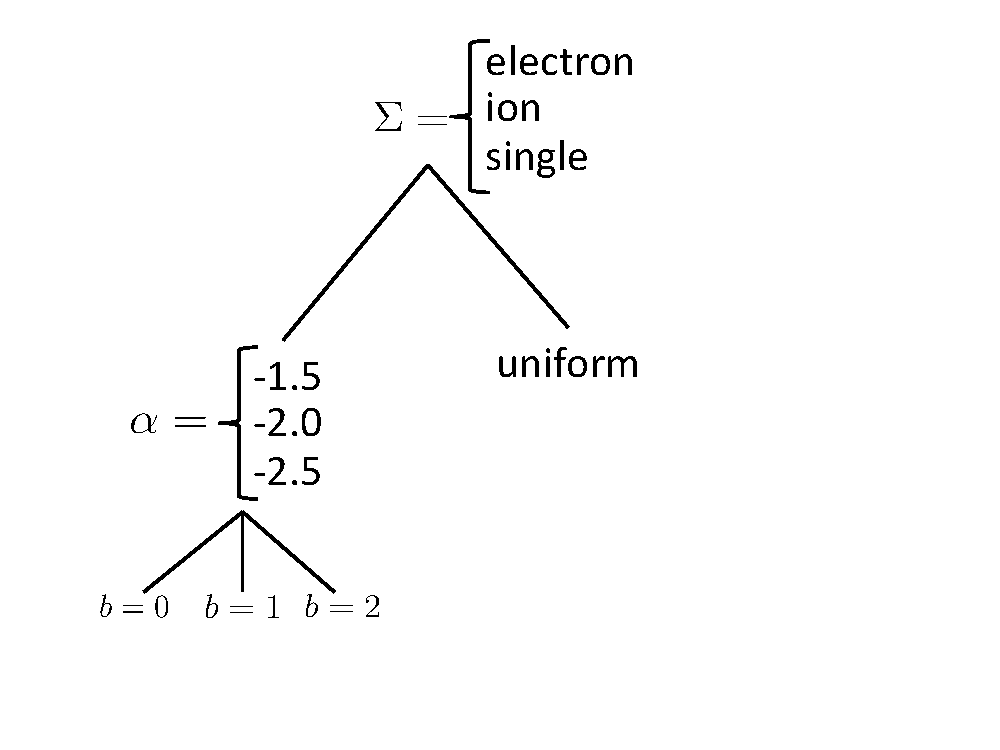
\includegraphics[width=0.6\columnwidth]{figures/parameter_space.pdf}
		\caption{Parameter space covered for each loop half-length $L$. $\alpha$ is the power-law index and $b$ indicates the scaling in the relationship $Q\propto T_N^b$, where $b=0$ corresponds to the case where $T_N$ and the event energy are independent.}
		\label{fig:parameter_space}
	\end{figure}
	%
	\begin{figure}
		\centering
		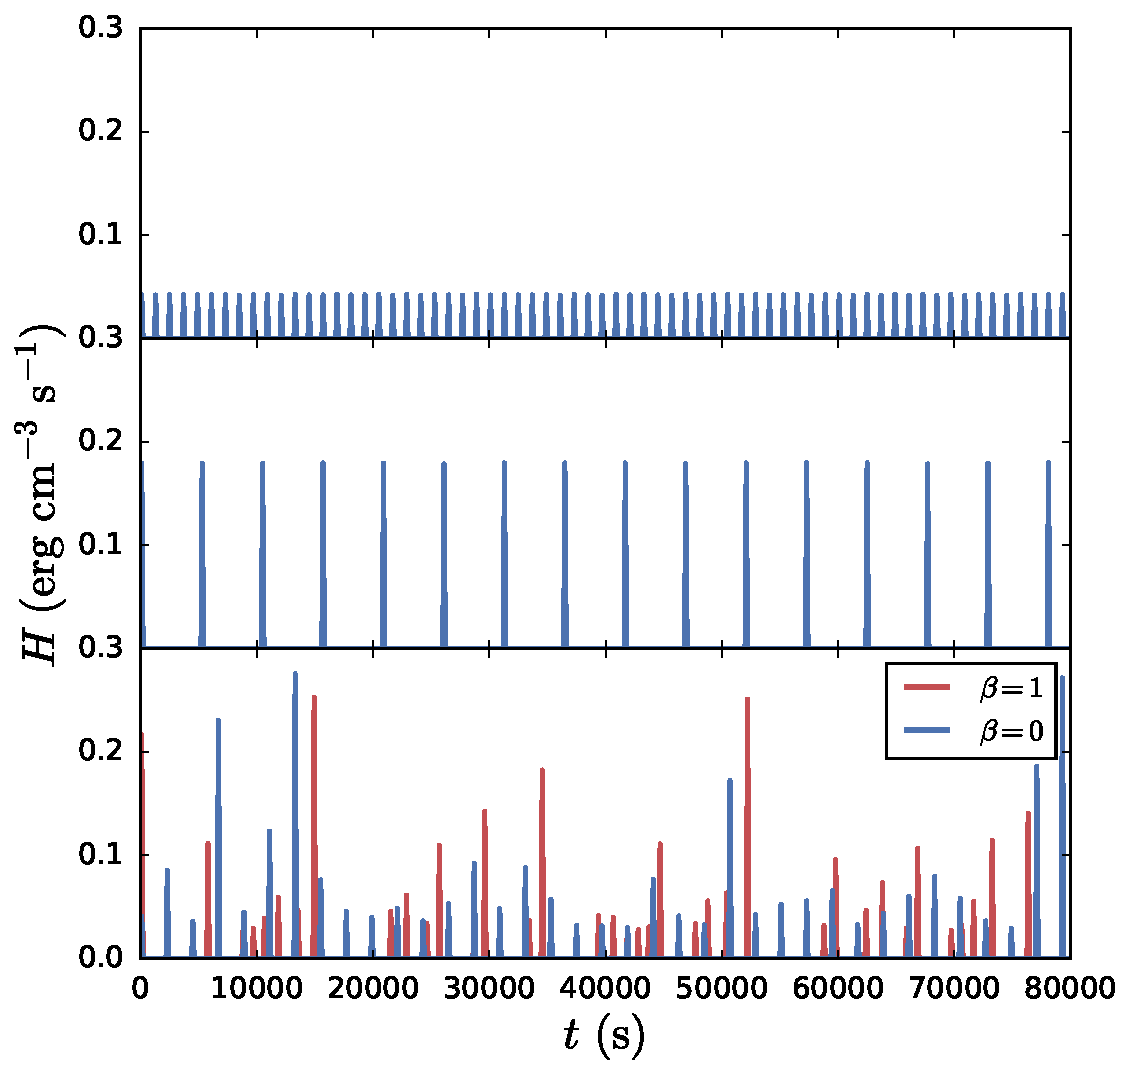
\includegraphics[width=\columnwidth]{figures/heating_functions.pdf}
		\caption{All heating functions are for $L=40$ Mm. Starting counter-clockwise from the bottom left: uniform heating amplitudes for $T_N=1000$ s; uniform heating amplitudes for $T_N=5000$ s; power-law distributed heating amplitudes for $\alpha=-1.5$, $T_N=2000$ s; power-law distributed amplitudes for $\alpha=-1.5$ where the wait times depend on the event energies and the mean wait time for both $b$ values is $\langle T_N\rangle=2000$ s.}
		\label{fig:heating_funcs}
	\end{figure}
	%
	\section{Results}
	%
	\subsection{Electron Heating}
	%
	\subsection{Ion Heating}
	%
	\subsection{Single-fluid}
	\section{Discussion}
	\section{Conclusion}
	
	%Bibliography
	\bibliography{references}
	\bibliographystyle{apj}
\end{document}